\documentclass{article}

\usepackage[utf8]{inputenc}
\usepackage[T1]{fontenc}
\usepackage{hyperref}
\usepackage{tabularx}
\usepackage{array}
\usepackage{fancyhdr}
\usepackage{graphicx}
\usepackage[a4paper]{geometry}
\usepackage{multicol}
\usepackage{listings}
\usepackage{tabto}

\title{Rapport de projet de JEE}
\author{par Jordan Baudin, Corentin Le Guen et Geoffrey Spaur}
\date{28 janvier 2018}
\pagestyle{fancy}
\lhead{Rapport de projet de JEE \\ \textbf{M2GIL} - Jordan Baudin, Corentin Le Guen et Geoffrey Spaur}
\rhead{
\includegraphics[scale=0.5]{logo_univ_rouen.png}}
\setlength{\headsep}{1cm}
\begin{document}

\maketitle
\newpage
\tableofcontents{}
\newpage
\section{Présentation}
  \paragraph{}
  Ce rapport à pour but d'apporter des réponses concernant le déroulement du projet, 
  ainsi que sur le résultat final et nos apprentissages tout au long du projet.
  
\newpage
\section{Implémentation de l'authentification}
  \paragraph{Le guide Spring} \
  
  Tout d'abord, il semblait plus faisable et raisonnable d'utiliser le guide Spring sur l'authentification
  pour écrire sur le sujet, mais le guide a montré uniquement de simples exemples, mais aucune véritable indication
  de systèmes fonctionnelles, avec enregistrement d'utilisateur et connexion, sans jamais montrer de gestion de session/token.
  Uniquement un utilisateur rentré en dur dans le code avec un rôle.

  \paragraph{Notre Implémentation} \
  
  Le choix a donc été de gérer les utilisateurs, rôles et tokens nous-mêmes.
  On ajoute donc un utilisateur lors d'une requête d'enregistrement (ou d'ajout par un administrateur, voir paragraphe sur la partie Administration),
  on vérifie si l'email est au bon format, si le mot de passe l'est aussi (a minima 8 caractères, une lettre minuscule, une lettre majuscule et un chiffre).
  Ensuite, on l'enregistre avec le rôle "USER".

  Lorsqu'une personne a un compte, il peut se connecter, il recevra alors un ID token, qu'il devra donner pour chacune des requêtes qu'il fera,
  pour vérifier qu'il est effectivement enregistré et connecté. Lorsque le cas est echéant, on vérifiera qu'il a le rôle nécessaire pour la requête faite.

  Pour modifier le rôle d'un utilisateur, il sera nécessaire de passer par l'Administration, donc seul un "ADMIN" pourra modifier ce rôle.

  La gestion du token se fait dans un module statique qui stocke les tokens valables en cours, si jamais le serveur tombe, tous les tokens deviennent caduques,
  afin d'éviter une attaque de vol de token. Le but ici est de privilégier la re-connexion de l'utilisateur à un token qui serait valable pendant 10 ans.
  On invalide le token lors d'une déconnexion.
  
\newpage
\section{Implémentation du Front}
  \paragraph{Choix de la technologie} \
  
  Nous avons choisi d'utiliser Angular4. Nous avons exclue Vue.js du choix des technologies
  car ce dernier est orienté MVVM (Modèle - Vue - Vue - Modèle), ce qui nous paraissait 
  inapproprié au projet demandé. De plus le framework Angular4 est recommandé dans le 
  travaille en groupe car c'est un framework orienté objet.
  
  \paragraph{Architecture en components} \
  
  Le framework Angular4 permet d'assembler un ensemble de composants entre eux. Ce
  framework permet de développer une application: \emph{single page application}.
  Chaque composant Angular4 est composé de plusieurs fichiers permettant en architecture MVC:\\ \\
  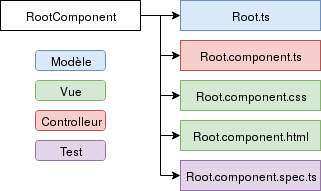
\includegraphics[scale=0.6]{archi_component.png}\\ \\
  Nous avons donc décomposé notre application avec ces composants:\\
  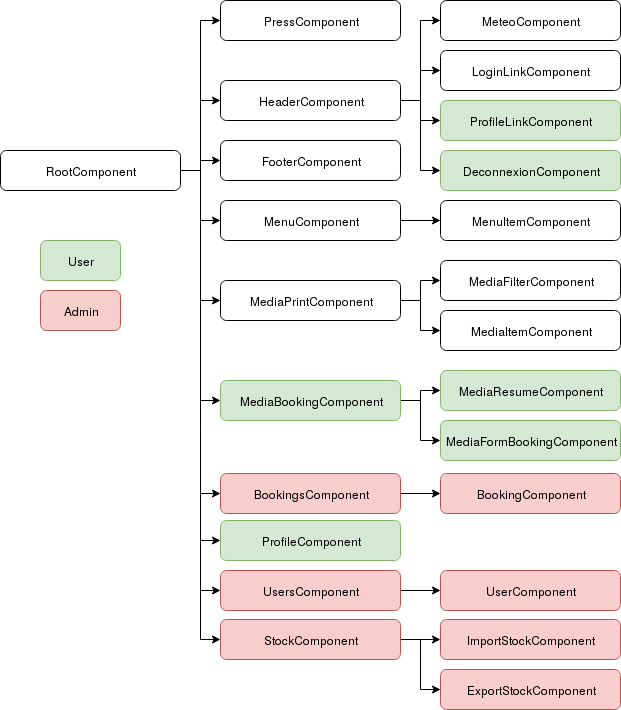
\includegraphics[scale=0.5]{allcomponent.png}
  
  \paragraph{Guide technique} \
  
  Angular4 permet de créer des applications qui seront hébergées sur un serveur node.js.
  Nous devons donc dans un premier temps installer ce serveur ainsi que le gestionnaire
  de package lié à node.js: npm. Vous trouverez les liens de téléchargement 
  \href{https://nodejs.org/en/download/}{ici}. Si vous êtes sur un système Linux,
  il est déconseillé d'utilisé les repos officiels. En effet ces derniers ne sont pas à jour,
  vous ne pourrez donc pas créer de projet angular4. téléchargez donc les binaires afin,
  de les inclure dans votre .bashrc. Puis vous devrez installer
  Angular CLI afin de pouvoir créer, modifier ou lancer votre projet:
  \begin{lstlisting}
  $ npm install -g @angular/cli
  \end{lstlisting}
  Vous pouvez donc maintenant créer un nouveau projet Angular avec la commande suivante:
  \begin{lstlisting}
  $ ng new frontend
  \end{lstlisting}
  Ainsi vous pourrez rajouter à loisir des composants à votre projet:
  \begin{lstlisting}
  $ ng generate component MenuComponent
  \end{lstlisting}
  Pour pouvoir lancer votre application, lancez la commande:
  \begin{lstlisting}
  $ ng serve
  \end{lstlisting}
  Vous pourrez ensuite parcourir votre application à l'adresse: \href{http://localhost:4200}{http://localhost:4200}

\end{document}